\documentclass[xetex,aspectratio=43]{beamer}

\usepackage{res/lections}

\preamble

\title[Основы схемотехники]{Физические и логические основы схемотехники}

\begin{document}

    \titleslide

    \tocslide


\section{Принципы действия активных электронных компонент}

\begin{frame}{Внимание!}
    \textbf{\alert{Внимание!\\
            Здесь надо смотреть и слушать лекцию, а не только слайды}}
\end{frame}

\subsection{Электромагнитные реле}

\begin{frame}{Электромагнитные реле}
    \url{https://en.wikipedia.org/wiki/Relay}
\end{frame}

\subsection{Ламповые диоды и триоды (I поколение)}

\begin{frame}{Закон Ома}
    \begin{figure}
        \includegraphics[height=0.75\textheight]{img/07.Ohm_Law.jpg}
    \end{figure}
    $$U = IR$$
\end{frame}

\begin{frame}{Электровакуумные элементы}

\begin{block}{Ламповые диоды и триоды }
\begin{itemize}
    \item \href{https://en.wikipedia.org/wiki/Vacuum_tube\#Diodes}{Диоды}
    \item \href{https://en.wikipedia.org/wiki/Vacuum_tube\#Triodes}{Триоды}
\end{itemize}
\end{block}

\begin{block}{Что мы узнаём?}
\begin{itemize}
    \item Термоэлектронная эмиссия
    \item Неуправляемый потенциальные барьер
    \item Управляемый потенциальные барьер
\end{itemize}

\end{block}


\pause

\begin{block}{Немного духа}
\begin{itemize}
    \item \href{https://youtu.be/DEewNHWgqFU}{Немного духа 1960-х}
    \item \href{https://youtu.be/EzyXMEpq4qw}{Немного викторианского духа в наши дни}
\end{itemize}

\end{block}

\end{frame}

\subsection[Полупроводниковые диоды и транзисторы, II+]{Полупроводниковые диоды и транзисторы (II и последующие поколения)}

\begin{frame}{Полупроводниковые элементы}

\begin{block}{Полупроводниковые диод и транзистор}
\begin{itemize}
\item
  \href{https://en.wikipedia.org/wiki/Diode}{Диод}
\item
  \href{https://en.wikipedia.org/wiki/Bipolar_junction_transistor}{Биполярный
  транзистор}
\end{itemize}
\end{block}

\pause

\begin{block}{Полупроводниковые диод и транзистор}
    \begin{itemize}
  \item \href{https://youtu.be/OMGdSCaMVD0?t=107}{Как оно вообще умудряется работать?..}
  \item \href{https://www.falstad.com/circuit/e-npn.html}{Симулятор}
    \end{itemize}
\end{block}

\pause

\begin{block}{Немного духа}
    \begin{itemize}
        \item \href{https://youtu.be/DEewNHWgqFU}{Немного духа 1960-х}
    \end{itemize}
\end{block}
\end{frame}

\section{Вентили}

\subsection{Вводная информация}

\begin{frame}{Что такое вентиль?}
\defn{Вентиль (gate)}{устройство, реализующее ту или иную логическую связку}

\pause

Вентили «не», «и», «или», «или-не» (NOR --- «not-or», \(\downarrow\))

\begin{figure}
    \includegraphics[width=1\textwidth]{img/07.gates_IEC.png}
    \caption{IEC / ГОСТ}
\end{figure}


\begin{figure}
    \includegraphics[width=1\textwidth]{img/07.gates_ANSI.png}
    \caption{ANSI}
\end{figure}

\end{frame}

\begin{frame}{История и экзотика: механические вентили}
\begin{itemize}
\item
  Компоненты машины Беббиджа
\item
  \href{http://bse.sci-lib.com/particle017859.html}{Пожаробезопасные и
  неизлучающие элементы универсальной системы элементов промышленной
  пневмоавтоматики}
\item
  \href{https://habr.com/ru/company/ruvds/blog/695210/}{Пневмоника} (в т.ч. \href{https://youtu.be/yvANcR4mQ7M}{самодельная})
\item
  \href{http://www.robives.com/category/product_tags/logic_goats}{Логические
  козлы}

  \begin{itemize}
  \item
    \href{https://youtu.be/vu3o6JNclRQ}{В действии}
  \end{itemize}
\end{itemize}
\end{frame}

\subsection{Электронные схемы вентилей}

\begin{frame}{Отрицание «с переключением»}
    \begin{figure}
        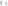
\includegraphics[height=0.5\textheight]{img/07.not_switch.pdf}
        \caption{Реле и транзисторно-транзисторная логика}
    \end{figure}
\end{frame}

\begin{frame}{Отрицание с согласующим резистором}
    \begin{figure}
        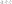
\includegraphics[height=0.5\textheight]{img/07.not_resist.pdf}
        \caption{Триод и резисторно-транзисторная логика}
    \end{figure}
\end{frame}

\begin{frame}{Как оно работает? (1)}
    \begin{figure}
        
\includegraphics[width=0.75\textwidth]{img/07.R-R.pdf}
    \end{figure}

\(I_\text{вх}\) и \(I_\text{вых}\) малы \(\implies\) \(I_{R_1} \approx I_{R_2}\).
Также \(\Delta_{U R1} / \Delta_{U R2} \approx R_1 / R_2\)

Легко вывести:
\[U_\text{вых} \approx \frac{U_H R_2 + U_L R_1}{R_1 + R_2}\]

Тогда: \(R_1 \ll R_2 \implies U_\text{вых} \approx U_H\) и \(R_1 \gg R_2 \implies U_\text{вых} \approx U_L\)
\end{frame}

\begin{frame}{Как оно работает? (2)}
    \begin{figure}
    \includegraphics[width=0.9\textwidth]{img/07.not_resist_physics.pdf}
    \caption{Пример для резисторно-транзисторной логики}
    \end{figure}
\end{frame}

\begin{frame}{Разные вентили}
    \begin{figure}
    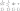
\includegraphics[width=0.9\textwidth]{img/07.transistor-gates.pdf}
    \end{figure}

    \begin{itemize}
    \tightlist
    \item
      Согласующие резисторы Везде, где схема может «не выдавать» сигнал
      (иногда с нулём)
    \item
      Диоды на входах, чтобы предотвратить распространение сигнала по
      входным линиям
    \end{itemize}
\end{frame}

\begin{frame}{Новости и не очень новости}
\begin{itemize}
\item
  2010: \href{https://www.science.org/doi/abs/10.1126/science.1192511}{Electromechanical Computing at 500°C with Silicon Carbide}
  Опытные микросхемы на основе карбида кремния (SiC)
  работают при $500-650 \textdegree{}C$, но медленные и жадные до питания.
  Альтернатива --- механические реле нанометрового масштаба.
\item
  2017: \href{https://www.nature.com/articles/ncomms15635}{Cascaded spintronic logic with low-dimensional carbon}
  Графеновые полевые транзисторы с большим быстродействием и широким диапазоном рабочих температур
\item
  2022: \href{https://singularityhub.com/2022/03/13/moores-law-scientists-just-made-a-graphene-transistor-gate-the-width-of-an-atom/}{Moore’s Law: Scientists Just Made a Graphene Transistor Gate the Width of an Atom}
  Транзистор рамером 0,34 нм.
\end{itemize}

\end{frame}

\section*{}

\begin{frame}{Вопросы и упражнения}
    \begin{block}{Вопросы}
        \begin{enumerate}
        \item
          Что такое логический вентиль?
        \item
          Постройте вентиль «не» на основе реле, триодов и транзисторов
        \item
          Постройте вентили «и», «или», «или-не» на основе транзисторов с
          согласующим резистором
        \end{enumerate}
    \end{block}

    \begin{block}{Упражнения}
    \begin{enumerate}
        \item Попробуйте спроектировать резисторно-транисторные элементы на основе PNP-транзисторов
    \end{enumerate}
\end{block}

\end{frame}

\postamble

\end{document}